%!TEX root = labo.tex

\chapter{Dynamic Routing Protocols (RIP and OSPF)}

What you will learn in this lab:
\begin{itemize}
	\item How to configure the routing protocols RIP, OSPF, and BGP on a Linux PC and a Cisco router.
	\item How those routing protocols update the routing tables after a change in the network topology.
	\item How the count-to-infinity problem in RIP can be avoided.
	\item How OSPF achieves a hierarchical routing scheme through the use of multiple areas.
\end{itemize}

\newpage
\setsession{prelab4}
\section{Prelab 4}\label{sec:prelab4}
%!TEX root = labo.tex

\subsubsection*{Routing protocols}
\begin{itemize}
	\item \emph{Distance Vector and Link State Routing Protocols}: Go to the website \url{http://docwiki.cisco.com/wiki/Internetworking_Technology_Handbook} and read the article about dynamic routing protocols. Review your knowledge of interdomain and intradomain routing, distance vector routing, and link state routing.
	\item \emph{Zebra}: Go to the website of the Zebra fork Quagga at \url{http://www.nongnu.org/quagga/} and study the information on the Quagga routing protocol software for Linux systems. Also find and read the man pages on zebra, ripd, ospfd and bgpd. Note: Quagga is a fork of the GNU Zebra project.
	\item \emph{RIP}: Read the overview of the Routing Information Protocol (RIP) and study the commands to configure RIP on a Cisco router at \url{http://www.routeralley.com/guides/rip.pdf}.
	\item \emph{OSPF}: Read the overview of Open Shortest Path First (OSPF) routing protocol and study the commands to configure OSPF on a Cisco router at \url{http://www.routeralley.com/guides/ospf.pdf}.
\end{itemize}

\newpage
\subsubsection*{Prelab Questions}

\begin{questions}
	\q{1}{Provide the command that configures a Linux PC as an IP router (see Lab 3).}
	\q{2}{What are the main differences between a distance vector routing protocol and a link state routing protocol? Give examples for each type of protocol.}
	\q{3}{What are the differences between an intradomain routing protocol (also called interior gateway protocol or IGP) and an interdomain routing protocol (also called exterior gateway protocol or EGP)? Give examples for each type of protocol.}
	\q{4}{Which routing protocols are supported by the software package Zebra?}
	\q{5}{In the Zebra software package, the processes ripd, ospfd, and bgpd deal, respectively, with the routing protocols RIP, OSPF, and BGP. Which role does the process zebra play?}
	\q{6}{Describe how a Linux user accesses the processes of Zebra (zebra, ripd, ospfd, bgpd) processes to configure routing algorithm parameters?}
	\q{7}{What is the main difference between RIP version 1 (RIPv1) and RIP version 2 (RIPv2)?}
	\q{8}{Explain what it means to ``run RIP in passive mode''.}
	\q{9}{Explain the meaning of ``triggered updates'' in RIP.}
	\q{10}{Explain the concept of split-horizon in RIP?}
	\q{11}{What is an autonomous system (AS)? Which roles do autonomous systems play in the Internet?}
	\q{12}{What is the AS number of your institution? Which autonomous system has AS number 1?}
	\q{13}{Explain the terms: Stub AS, Multi-homed AS and Transit AS?}
\end{questions}


\newpage
\setsession{lab4}
\section{Lab 4}\label{sec:lab4}

In the previous lab, you learned how to configure routing table entries manually. This was referred to as static routing. The topic of Lab 4 is dynamic routing, where dynamic routing protocols (from now on, called routing protocols) set the routing tables automatically without human intervention. Routers and hosts that run a routing protocol, exchange routing protocol messages related to network paths and node conditions, and use these messages to compute paths between routers and hosts.

Most routing protocols implement a shortest-path algorithm, which, for a given set of routers, determines the shortest paths between the routers. Some routing protocols allow that each network interface be assigned a cost metric. In this case, routing protocols compute paths with least cost. Based on the method used to compute the shortest or least-cost paths, one distinguishes distance vector and link state routing protocols. In a distance vector routing protocol, neighbouring routers send the content of their routing tables to each other, and update the routing tables based on the received routing tables. In a link state routing protocol, each router advertises the cost of each of its interfaces to all routers in the network. Thus, all routers have complete knowledge of the network topology, and can locally run a shortest-path (or least-cost) algorithm to determine their own routing tables.

The notion of an autonomous system (AS) is central to the understanding of routing protocols on the Internet. An autonomous system is a group of IP networks under the authority of a single administration, and the entire Internet is carved up into a large number of autonomous systems. Examples of autonomous systems are the campus network of a university and the backbone network of a global network service provider. Each autonomous system is assigned a globally unique identifier, called the AS number. On the Internet, dynamic routing within an autonomous system and between autonomous systems is handled by different types of routing protocols. A routing protocol that is concerned with routing within an autonomous system is called an intradomain routing protocol or interior gateway protocol (IGP). A routing protocol that determines routes between autonomous systems is called an interdomain routing protocol or exterior gateway protocol (EGP).

In this lab, you study the two most common intradomain protocols, namely, the Routing Information Protocol (RIP) and the Open Shortest Path First (OSPF) protocol. Parts 1-3 of this lab deal with RIP, and Parts 4-5 are about OSPF. 
% In Part 7, you are exposed to a few features of the Border Gateway Protocol (BGP), which is the interdomain routing protocol of the Internet.

This lab uses two different network configurations. The first network configuration, shown in Figure \ref{fig:lab4-network1}, is used in Parts 1-2, and is modified in Part 3 (Figure \ref{fig:lab4-network1-part3}). The network configuration in Parts 4 and 5 is shown in Figure \ref{fig:lab4-network2}.

\newpage
\subsection{Configuring RIP on a Cisco router}

This lab starts with the same network topology as used in Part 5 of Lab 3. Different from Lab 3, where the routing tables were configured manually, here you run the routing protocol RIP to perform the same task. In Part 1, you configure RIP on the Cisco routers. In Part 2, you configure RIP on the Linux PCs.

RIP is one of the oldest dynamic routing protocols on the Internet that is still in use. This lab uses the latest revision of RIP, RIPv2 (RIP version 2). RIP is an intradomain routing protocol that uses a distance vector approach to determine the paths between routers. RIP minimizes the number of hops of each path, where each point-to-point link or LAN constitutes a hop.

Each RIP enabled router periodically sends the content of its routing table to all its neighbouring routers in an update message. For each routing table entry, the router sends the destination (host IP address or network IP address) and the distance to that destination measured in hops. When a router receives an update message from a neighbouring router, it updates its own routing table.

Figure \ref{fig:lab4-network1} and Table \ref{tab:lab4-network1} describe the network configuration for this part of the lab.

\begin{figure}[ht]
	\centering
	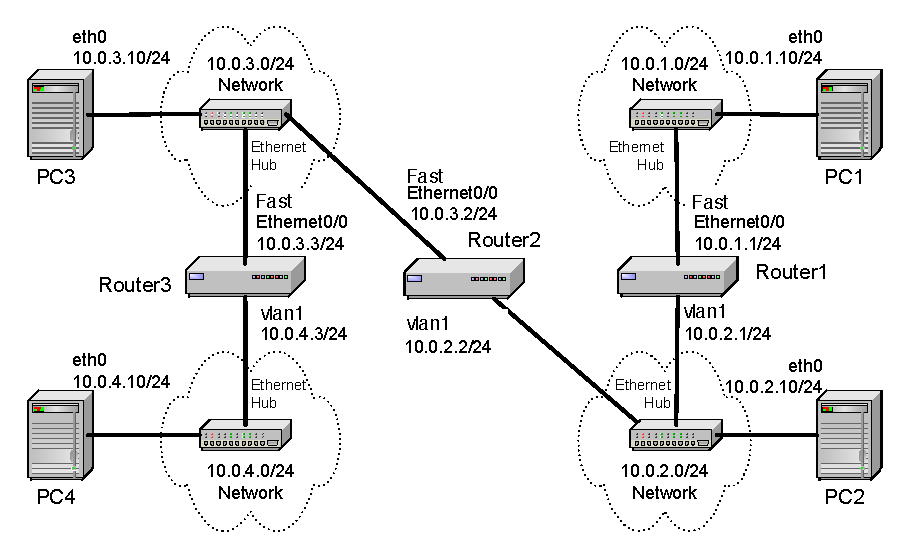
\includegraphics[width=\linewidth]{graphics/lab4-network1-updated.pdf}	
	\caption{Network configuration for Parts 1 and 2.}
	\label{fig:lab4-network1}
\end{figure}

\begin{table}[h!t]
	\centering
	\begin{tabular}{| c | c | c |}	
		\hline
		\textbf{Linux PC} & \textbf{eth0} & \textbf{eth1} \\ \hline
		PC1 & 10.0.1.10/24 & Disabled \\ 
		PC2 & 10.0.2.10/24 & Disabled \\
		PC3 & 10.0.3.10/24 & Disabled \\
		PC4 & 10.0.4.10/24 & Disabled \\ \hline
		\textbf{Cisco Router} & \textbf{FastEthernet0/0} & \textbf{vlan1} \\ \hline
		Router1 & 10.0.1.1/24 & 10.0.2.1/24 \\
		Router2 & 10.0.3.2/24 & 10.0.2.2/24 \\
		Router3 & 10.0.3.3/24 & 10.0.4.3/24 \\ \hline
	\end{tabular}
	\caption{IP addresses}
	\label{tab:lab4-network1}
\end{table}

\subsubsection*{Exercise 1. Configuring RIP on Cisco routers}

Configure all three Cisco routers to run the routing protocol RIP. Once the configuration is completed, all Cisco routers can issue ping commands to each other. Below, we give a brief overview of the basic commands used to configure RIP on a Cisco router.

The following can can be executed in the Global Configuration mode.

\begin{itemize}
	\item Enable the routing protocol RIP on the local router, and enters the router configuration mode from the following prompt:
		\begin{cmdblock}
	Router1(config-router)#
		\end{cmdblock}
		You return from the router configuration command to the global configuration command by typing the command \cmd{exit}.
		\begin{cmdblock}
	router rip
		\end{cmdblock}
	\item Disable RIP on the local router.
		\begin{cmdblock}
	no router rip
		\end{cmdblock}
\end{itemize}

The following can can be executed in the Privileged EXEC mode.

\begin{itemize}
	\item Enable a debugging mode where the router displays a message for each received RIP packet.
		\begin{cmdblock}
	debug ip rip
		\end{cmdblock}
	\item Disable the debugging feature
		\begin{cmdblock}
no debug ip rip
		\end{cmdblock}
\end{itemize}

The following can can be executed in the Router Configuration mode.

\begin{itemize}
	\item Associate the network IP address \emph{Netaddr} with RIP. RIP sends updates only on interfaces where the network address has been associated with RIP.
		\begin{cmdblock}
network Netaddr
		\end{cmdblock}
	\item Disable RIP for the specified network address.
		\begin{cmdblock}
	no network Netaddr
		\end{cmdblock}
	\item Set the interface \emph{Iface} in RIP passive mode. On an interface in passive mode, the router processes incoming RIP packets, but does not transmit RIP packets.
		\begin{cmdblock}
	passive-interface Iface
		\end{cmdblock}
	\item Enable active mode on interface \emph{Iface}. This means that RIP packets are transmitted on this interface.
		\begin{cmdblock}
	no passive-interface Iface
		\end{cmdblock}
	\item Increase the metric (hop count) of incoming RIP packets that arrive on interface \emph{Iface} by \emph{value}, where \emph{value} is a number.
		\begin{cmdblock}
	offset-list 0 in value Iface
		\end{cmdblock}
	\item Increase the metric of outgoing RIP packets that are sent on interface \emph{Iface} by \emph{value}.
		\begin{cmdblock}
	offset-list 0 out value Iface
		\end{verbatim}
	\item Disable the specified offset-list command for incoming RIP packets.
		\begin{cmdblock}
	no offset-list 0 in value Iface
		\end{cmdblock}
	\item Disable the specified offset-list command for outgoing RIP packets.
		\begin{cmdblock}
	no offset-list 0 out value Iface
		\end{cmdblock}
	\item Set the RIP version to RIPv2.
		\begin{cmdblock}
	version 2
		\end{cmdblock}
	\item Set the values of the timers in the RIP protocol. The timers are measured in seconds.
		\begin{cmdblock}
	timers basic update invalid hold-down flush
		\end{cmdblock}
		\begin{description}
			\item [\texttt{update}]: The time interval between transmissions of RIP update messages (Default: 30 sec).
			\item [\texttt{invalid}]: The time interval after which a route, which has not been updated, is declared invalid (Default: 180 sec).
			\item [\texttt{hold-down}]: Determines how long after a route has been updated as unavailable, a router will wait before accepting a new route with a lower metric. This introduces a delay for processing incoming RIP packets with routing updates after a link failure (Default: 180 sec).
			\item [\texttt{flush}]: The amount of time that must pass before a route that has not been updated is removed from the routing table (Default: 240 sec).
		\end{description}
		Example:
		\begin{cmdblock}
	Router1(config-router)# timers basic 30 180 180 240
		\end{cmdblock}
	\item Set the router to not perform triggered updates, when the next transmission of routing updates is due in time. If time is set to the same value as the update timer, then triggered updates are disabled. In RIP, a triggered update means that a router sends a RIP packet with a routing update, whenever one of its routing table entries changes.
		\begin{cmdblock}
	flash-update-threshold time
		\end{cmdblock}
\end{itemize}

\begin{enumerate}
	\item Connect the the Linux PCs and the Cisco routers as shown in Figure \ref{fig:lab4-network1}. The PCs and routers are connected with Ethernet hubs.
	\item Verify that the serial interfaces of the PCs are connected to the console port of the routers. PC1 should be connected to Router1, PC2 to Router2, and so on. Once the serial cables are connected, establish a minicom session from each PC to the connected router.
	\item On Router1, Router2, and Router3, configure the IP addresses as shown in Table \ref{tab:lab4-network1}, and enable the routing protocol RIP. The commands to set up Router1 are as follows:
		\begin{cmdblock}
	Router1> enable Password: <enable secret>
	Router1# configure terminal
	Router1(config)# no ip routing
	Router1(config)# ip routing
	Router1(config)# router rip
	Router1(config-router)# version 2 
	Router1(config-router)# network 10.0.0.0 
	Router1(config-router)# interface FastEthernet0/0 
	Router1(config-if)# no shutdown
	Router1(config-if)# ip address 10.0.1.1 255.255.255.0 
	Router1(config-if)# interface FastEthernet0/1 
	Router1(config-if)# no shutdown
	Router1(config-if)# interface vlan1
	Router1(config-if)# no shutdown
	Router1(config-if)# ip address 10.0.2.1 255.255.255.0 
	Router1(config-if)# end
	Router1# clear ip route *
		\end{cmdblock}
		The command \cmd{no ip routing} is used to reset all previous configurations related to routing (RIP, OSPF, etc). The command \cmd{clear ip route *} deletes all entries in the routing table. Make sure that all static routing entries are removed, since, in IOS, RIP does not overwrite static routing entries.
	\item After you have configured the routers, check the routing table at each router by typing
		\begin{cmdblock}
	Router1# show ip route
		\end{cmdblock}
		Each router should have four entries in the routing table: two entries for directly connected networks, and two other entries for remote networks that were added by RIP.
	\item From each router, issue a ping command to the IP addresses of interfaces \iface{FastEthernet0/0} and \iface{vlan1} on all remote routers. For example, to issue a ping from Router1 to interface \iface{FastEthernet0/0} on Router2, type
		\begin{cmdblock}
	Router1# ping 10.0.3.2
		\end{cmdblock}
\end{enumerate}

Once you can successfully contact the IP addresses of all routers, proceed to the next exercise.

\newpage
\subsection{Configuring RIP on a Linux PC}

In this part of the lab, you continue with the network configuration in Figure \ref{fig:lab4-network1} and Table \ref{tab:lab4-network1}, and configure RIP on the Linux PCs.

In Figure \ref{fig:lab4-network1}, all Linux PCs are set up as hosts. Since hosts do not perform IP forwarding, they need not send routing messages. Therefore, when a routing protocol is configured on a host, the protocol is set to run in passive mode, where a host receives and processes incoming routing messages, but does not transmit routing messages. (We note that, normally, routing protocols are not enabled on hosts. Instead, one generally configures a static routing table entry for the default gateway. Obviously, when a routing protocol is enabled, there is no need to configure a default gateway.)

The configuration of routing protocols on Linux PCs in Lab 4 is done with the routing software package Quagga. Before starting the exercise, we give a brief tutorial on the Quagga software package. The tutorial focuses on the features used in the lab exercises and omits many interesting features of Zebra.

\subsubsection*{An Introduction to Quagga}

Quagga is a software package that manages the routing tables of a Linux system, and that provides the ability to execute a variety of routing protocols. For this course we make use of Quagga, which is a fork of the GNU Zebra project and while the project has a new name, many of the references to Zebra still remain, e.g. there is still a \cmd{zebra} control process.

The Quagga architecture, shown in Figure \ref{fig:quagga}, consists of a set of processes. The process \cmd{zebra} updates the routing tables and exchanges routes between different routing protocols. Each routing protocol has a separate process, and each routing process can be started, stopped, configured, and upgraded independently of the other routing processes. The process \cmd{zebra} must be invoked prior to starting and configuring any of the routing protocols. The routing processes used in this lab and the routing protocols they manage are shown in table \ref{tab:quagga}.

\begin{table}[h!t]
	\centering
	\begin{tabular}{| l l |}	
		\hline
		\textbf{Routing Process} & \textbf{Routing Protocol}\\ \hline
		ripd & RIPv1 and RIPv2 \\
		ospfd & OSPFv2 (Version 2) \\ \hline
	\end{tabular}
	\caption{Quagga routing processes used for this lab.}
	\label{tab:quagga}
\end{table}

\begin{figure}[h]
	\centering
	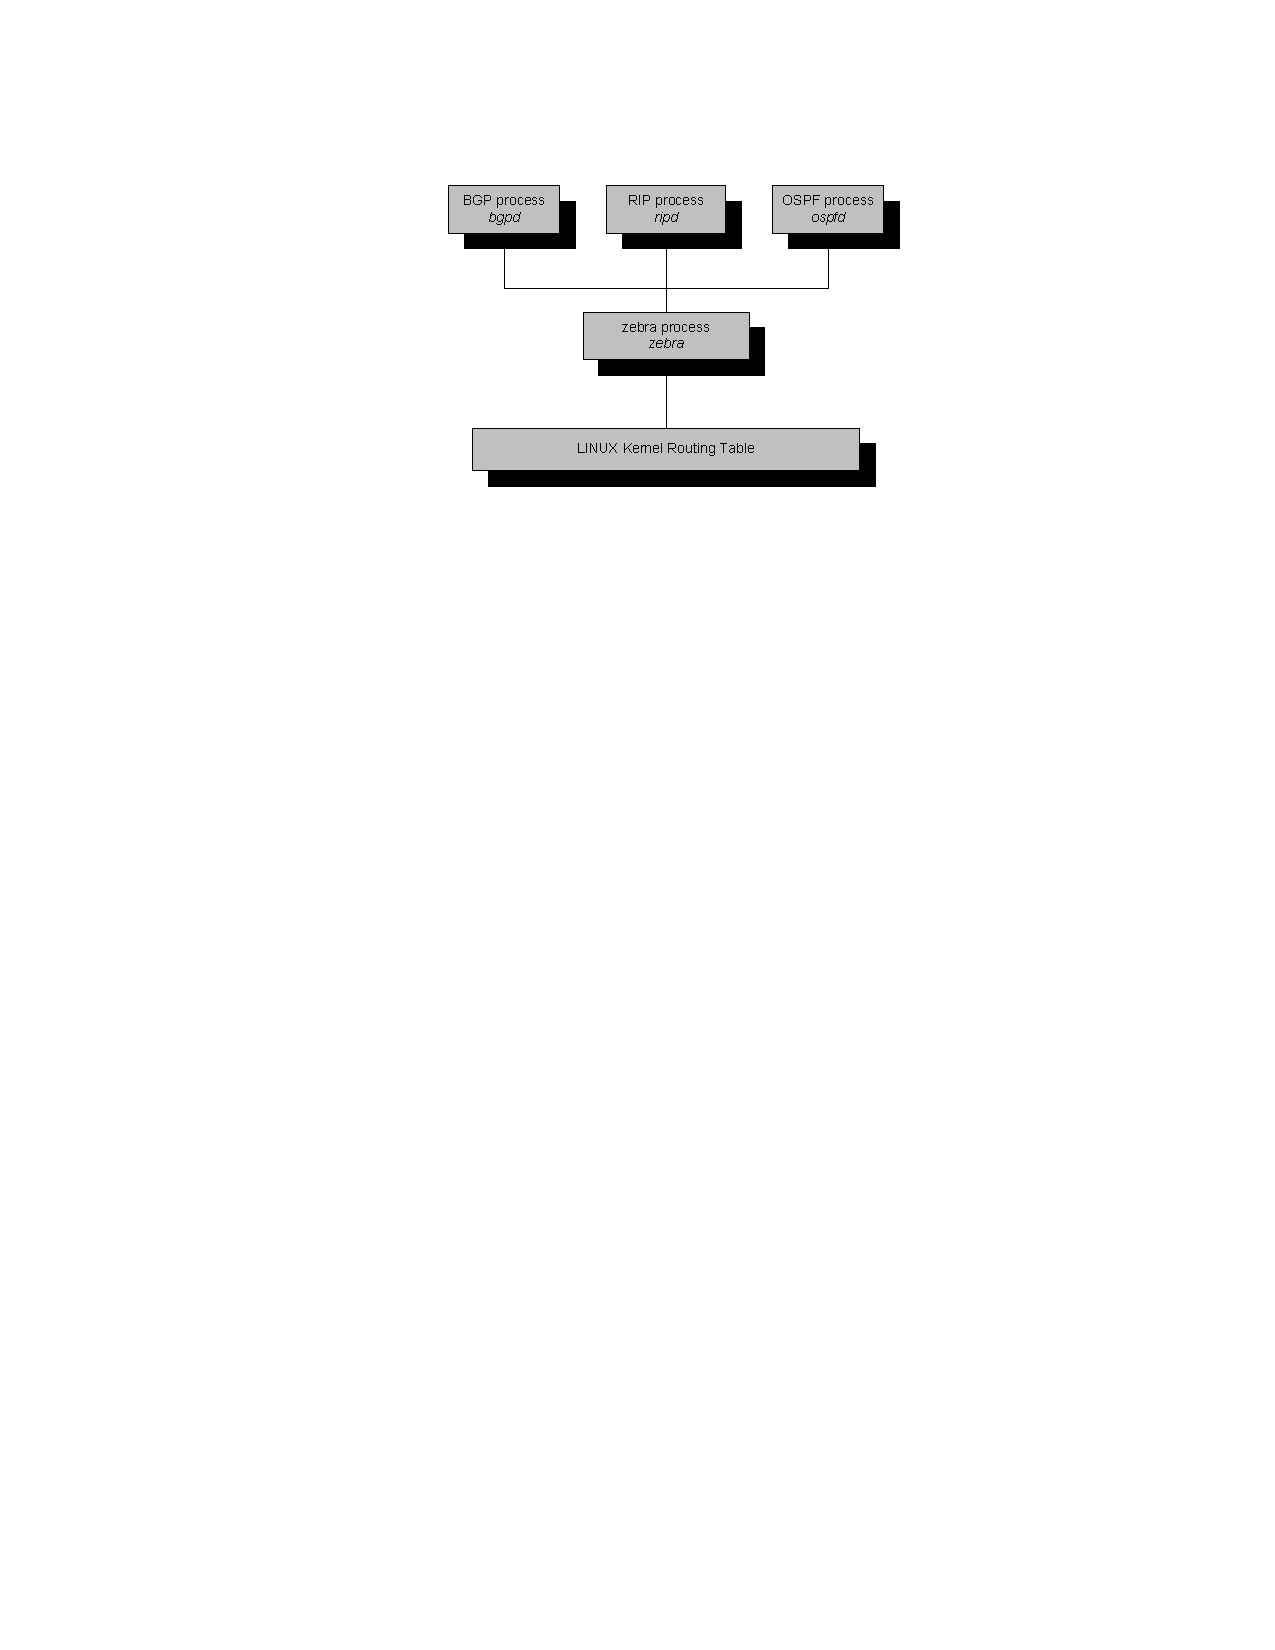
\includegraphics[width=0.7\linewidth]{graphics/quagga.pdf}	
	\caption{Quagga processes}
	\label{fig:quagga}
\end{figure}

\begin{enumerate}[label=\textbf{(\alph*)},labelindent=0em]
	\item \textbf{Adding the directory with Quagga commands to the search path}\hfill \\
		On Ubuntu systems, the script to start, stop and control the \cmd{zebra} process and its routing processes is located in directory \path{/etc/init.d}. % and can be called by means of the \cmd{service} command:
		\begin{cmdblock}
	PC1% /etc/init.d/quagga start
		\end{cmdblock}

	\item \textbf{Starting and stopping Quagga processes}
		\begin{description}
			\item[\texttt{/etc/init.d/quagga start}]\hfill \\
				Start the Quagga processes.
			\item[\texttt{/etc/init.d/quagga stop}]\hfill \\
				Terminate the Quagga processes.
			\item[\texttt{/etc/init.d/quagga restart}]\hfill \\
				Stop and restart the Quagga processes.
		\end{description}
		To set up a routing process, you must enable the routing daemon in the Quagga configuration file \path{/etc/quagga/daemons} and than start the \cmd{quagga} service. For example to start the RIP routing protocol daemon, your \path{daemons} file should look as shown below. Afterwards, you can start the \cmd{zebra} and the \cmd{ripd} daemons by running \cmd{/etc/init.d/quagga start} or \cmd{/etc/init.d/quagga restart} in case Quagga was already running.
		\begin{cmdblock}
	zebra=yes
	bgpd=no
	ospfd=no
	ospf6d=no
	ripd=yes
	ripngd=no
	isisd=no
		\end{cmdblock}
		Make sure the \cmd{zebra} daemon is always enabled as the other routing daemons depend on this process. When you type \cmd{/etc/init.d/quagga stop}, then all routing protocol processes are stopped as well.

		For the \cmd{zebra} process and all other routing processes, there is a configuration file which is read when the process is started. The configuration files are located in the directory \path{/usr/local/etc} or \path{/etc/quagga}, and have names \path{zebra.conf}, \path{ripd.conf}, etc. The configuration files look similar to the configuration files of IOS, and contain commands that are executed when the process is started.

	\item \textbf{Configuring the \cmd{zebra} process and the routing protocol processes}\hfill \\
		After starting the \cmd{zebra} process or any of the routing protocol processes, you can configure each process by establishing a Telnet session to that process. Each process listens on a specific port for incoming requests to establish a Telnet session. The port numbers of the processes are as follows:
		\begin{itemize}
			\item 2601 - Zebra
			\item 2602 - ripd
			\item 2604 - ospfd
		\end{itemize}
		If you establish a Telnet session to a routing process, you are asked for a password. If the password is correct, a command prompt is displayed. For example, to access the ripd process on the local host you type:
		\begin{cmdblock}
	PC1% telnet localhost 2602
		\end{cmdblock}
		This results in the following output.
		\begin{cmdblock}
	Trying 127.0.0.1...
	Connected to localhost.
	Escape character is '^]'.
	
	Hello, this is Quagga (version 0.99.20.1).
	Copyright 1996-2005 Kunihiro Ishiguro, et al.
	
	
	User Access Verification
	
	Password: <enter password>
	ripd>
		\end{cmdblock}
		At the prompt, you may type configuration commands. The Telnet session is terminated with the command
		\begin{cmdblock}
	ripd> exit
		\end{cmdblock}
	\item \textbf{Typing configuration commands}\hfill \\
		Once you have established a Telnet session to a routing process, you can configure the routing protocol of that process. The command line interface of the routing processes emulates the IOS command line interface, that is, the processes have similar command modes as IOS, and the syntax of commands is generally the same as the corresponding commands in IOS.
For example, the following commands configure the RIP routing protocol for network 10.0.0.0/8 on a Linux PC.
		\begin{cmdblock}
	ripd> enable
	ripd# configure terminal
	ripd(config)# router rip 
	ripd(config-router)# version 2 
	ripd(config-router)# network 10.0.0.0/8 
	ripd(config-router)# end
	ripd# exit
		\end{cmdblock}
		The password and enable password for all Quagga deamons (ripd and ospfd) is set to `mvkbj1n`.
\end{enumerate}

After this brief tutorial, you can now complete the configuration of RIP on the Linux PCs.

\subsubsection*{Exercise 2. Configuring RIP on Linux PCs with Quagga}

Enable RIP on all Linux PCs. Since all Linux PCs are running as hosts, RIP is set to passive mode, where the PCs receive and process incoming RIP packets, but do not transmit RIP packets. The following guidelines describe the configuration of PC1. Repeat the steps on each PC.

\begin{enumerate}
	\item On PC1, start the \cmd{zebra} and the\cmd{ripd} daemons by typing 
		\begin{cmdblock}
	PC1% /etc/init.d/quagga start
		\end{cmdblock}
		Make sure your \path{daemons} configuration file is correctly configured.
	\item To configure the RIP routing process on PC1, connect to the \cmd{ripd} process via Telnet.
		\begin{cmdblock}
	PC1% telnet localhost 2602
		\end{cmdblock}
		The system will prompt you for a login password. The password should be the same password as the login password on the Cisco routers.
	\item The Linux PCs, which are configured as hosts, will be set to run RIP in passive mode. The commands to enable RIP in passive mode are as follows:
		\begin{cmdblock}
	ripd> enable
	ripd# configure terminal
	ripd(config)# router rip 
	ripd(config-router)# version 2 
	ripd(config-router)# network 10.0.0.0/8 
	ripd(config-router)# passive-interface eth0 
	ripd(config-router)# end
	ripd# show ip rip
		\end{cmdblock}
		The \cmd{show ip rip} displays the routing database of the RIP protocol. This command does not exist in IOS. It may take a few minutes until RIP has built up its routing database. When the routing table has stabilized, that is, the results of the command \cmd{show ip rip} do not change after subsequent rounds of update messages, save the output of the command, and exit the Telnet session with the command.
		\begin{cmdblock}
	ripd# exit
		\end{cmdblock}
	\item On PC1, view the routing table with the command
		\begin{cmdblock}
	PC1% netstat -rn
		\end{cmdblock}
		and save the output to a file.
		Compare the output of \cmd{netstat -rn} to the output of \cmd{show ip rip}. Note the cost metric for each entry.
	\item Repeat Steps 1-5 for the other three Linux PCs.
	\item Once you can successfully issue a ping from each Linux PCs to every other Linux PC, display the route from PC1 to PC4 (10.0.4.10) with the \cmd{traceroute} command and save the result to a file:
		\begin{cmdblock}
	PC1% traceroute 10.0.4.10
		\end{cmdblock}
	\item Start to capture traffic with Wireshark on all four Linux PCs. Set a capture filter or display filter to display only RIP packets.
	\item Stop the traffic Wireshark capture on the PCs and save the traces for your report to a pcap file. Save the content of those RIP messages, needed to answer the questions in Part 8 (Select the Print details option).
\end{enumerate}

\begin{questions}
	\q{2.1}{Use the captured data of a single RIP packet and explain the fields in a RIP message.}
	\q{2.2}{For PC1, include the output of the commands \cmd{show ip rip} and \cmd{netstat -rn} from Steps 4 and 5. Discuss the differences in the output of the commands.}
	\q{2.3}{Include the output of \cmd{traceroute} from Step 7.}
	\q{2.4.a}{What is the destination IP address of RIP packets?}
	\q{2.4.b}{Do routers forward RIP packets? In other words, does PC1 receive RIP packets sent by Router3?}
	\q{2.4.c}{Which types of routing RIP messages do you observe? The type of a RIP message is indicated by the value of the field command. For each packet type that you observed, explain the role that this message type plays in the RIP protocol.}
	\q{2.4.d}{A RIP message may contain multiple routing table entries. How many bytes are consumed in a RIP message for each routing table entry? Which information is transmitted for each message?}
\end{questions}

\newpage
\subsection{Reconfiguring the topology in RIP}

In Part 3, you add Router4 to the network topology of Figure \ref{fig:lab4-network1}. The configuration of the network with Router4 is illustrated in Figure \ref{fig:lab4-network1-part3}. The IP configuration of Router4 is given in Table \ref{tab:lab4-network1-part3}. The purpose of this exercise is to explore how RIP detects changes to the network topology, and how long it takes until RIP updates the routing tables.

\begin{figure}[ht]
	\centering
	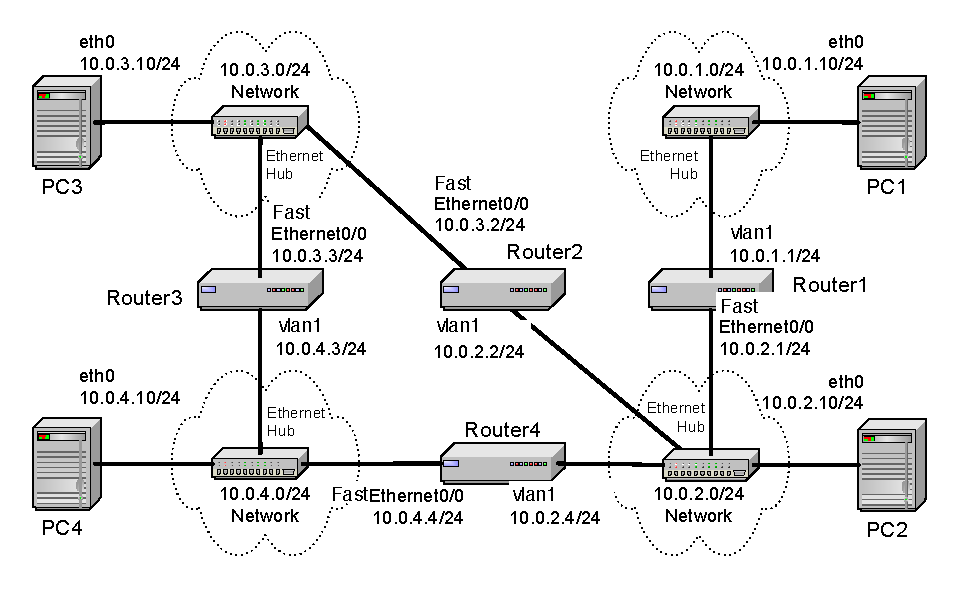
\includegraphics[width=\linewidth]{graphics/lab4-network1-part3-updated.pdf}	
	\caption{Network configuration for Part 3.}
	\label{fig:lab4-network1-part3}
\end{figure}

\begin{table}[h!t]
	\centering
	\begin{tabular}{| c | c | c |}	
		\hline
		\textbf{Cisco Router} & \textbf{FastEthernet0/0} & \textbf{vlan1} \\ \hline
		Router4 & 10.0.4.4/24 & 10.0.2.4/24 \\ \hline
	\end{tabular}
	\caption{IP addresses of Router4}
	\label{tab:lab4-network1-part3}
\end{table}

\subsubsection*{Exercise 3-A. Updating the routing tables}

Add Router4 to the network and observe the routing table updates made by RIP to reflect the new topology.

\begin{enumerate}
	\item Continue with the network configuration of Part 2. RIP must be enabled on all Routers shown in Figure \ref{fig:lab4-network1}, and a RIP process must be running (in passive mode) on all Linux PCs.
	\item Before attaching Router4, save the routing tables on all four Linux PCs with the command \cmd{netstat -rn}.
	\item Connect Router4 as shown in Figure \ref{fig:lab4-network1-part3} and assign the IP addresses to the interfaces as shown in Table \ref{tab:lab4-network1-part3}.
	\item Configure Router4 to run RIP, following the same steps as in Part 1.
	\item Use the command \cmd{netstat -rn} on the Linux PCs to observe how the routing tables are updated. Once the routing tables on the PCs have converged, save the routing tables on all four Linux PCs.
\end{enumerate}

\begin{questions}
	\q{3.A}{Include the routing tables of the Linux PCs before the topology was changed (Step 2) and after Router4 has been added and the routing tables have been updated (Step 5). Discuss the time it took to update the routing tables.}
\end{questions}

\subsubsection*{Exercise 3-B. Convergence of RIP after a link failure}

Next you disconnect the Ethernet cable of interface Ethernet0/0 on Router4 and observe how much time RIP takes to update the routing table of the Linux PCs to reflect the new topology.

\begin{enumerate}
	\item Issue a \cmd{ping} command from PC4 to PC1. Do not terminate the \cmd{ping} command until this exercise is completed in Step 4.
		\begin{cmdblock}
	PC4% ping 10.0.1.10
		\end{cmdblock}
	\item Disconnect the Ethernet cable connected to interface \iface{FastEthernet0/0} on Router4. Now, the output of ping on PC4 should show that the destination network is unreachable.
	\item Wait until the ping command is successful again, that is, ICMP Echo Reply messages arrive at PC4. This occurs once an alternate path has been found between PC4 and PC1, and the routing tables have been updated accordingly. This may take several minutes.
	\item Stop the ping command with \cmd{Ctrl-c} and save the ping statistics output (i.e. the data that appears at the bottom of the terminal screen when you stop the ping process).
	\item Count the number of lost packets and calculate the time it took RIP to update the routing tables. (The \cmd{ping} command issues an ICMP Echo Request message approximately once every second.)
\end{enumerate}

\begin{questions}
	\q{3.B}{Include your answer on the convergence time from Step 4. Count the number of lost packets and calculate the time it took RIP to update the routing tables. (The ping command issues an ICMP Echo Request message approximately once every second.)}
\end{questions}

\newpage
\subsection{Configuring Open Shortest Path First (OSPF)}

Next, you explore the routing protocol Open Shortest Path First (OSPF). OSPF is a link state routing protocol, where each router sends information on the cost metric of its network interfaces to all other routers in the network. The information about the interfaces is sent in messages that are called link state advertisements (LSAs). LSAs are disseminated using flooding, that is, a router sends its LSAs to all its neighbours, which, in turn, forward the LSAs to their neighbours, and so on. However, each LSA is forwarded only once. Each router maintains a link state database of all received LSAs, which provides the router with complete information about the topology of the network. Routers use their link state databases to run a shortest path algorithm that computes the shortest paths in the network.

Unlike distance vector routing protocols, link state routing protocols do not have convergence problems, such as the count-to-infinity problem. This is seen as a significant advantage of link state protocols over distance vector protocols.

OSPF is the most important link state routing protocol on the Internet. The functionality of OSPF is rich, and the lab exercises highlight only a small portion of the OSPF protocol. The Internet Lab uses OSPF version 2 (OSPFv2).
The network configuration is shown in Figure \ref{fig:lab4-network2} and Table \ref{tab:lab4-network2}. Note that some Linux PCs and routers are connected with crossover cables.

\begin{figure}[ht]
	\centering
	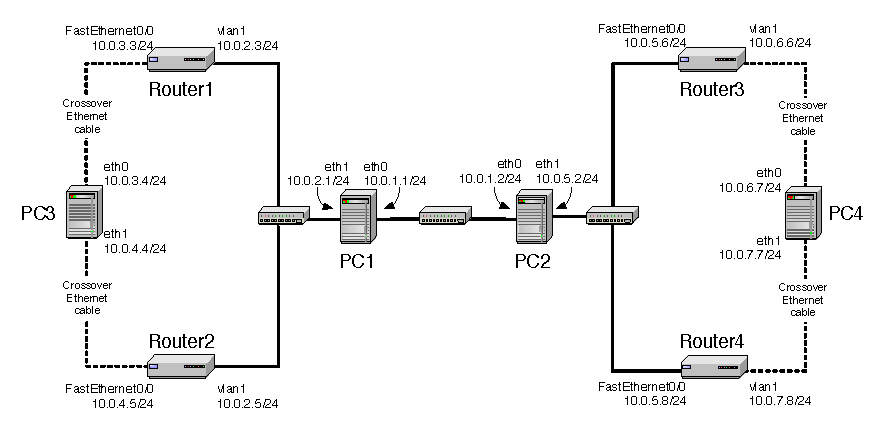
\includegraphics[width=\linewidth]{graphics/lab4-network2-updated.pdf}	
	\caption{Network configuration for Part 4.}
	\label{fig:lab4-network2}
\end{figure}

\begin{table}[h!t]
	\centering
	\begin{tabular}{| c | c | c |}	
		\hline
		\textbf{Linux PC} & \textbf{eth0} & \textbf{eth1} \\ \hline
		PC1 & 10.0.1.1/24 & 10.0.2.1/24 \\ 
		PC2 & 10.0.1.2/24 & 10.0.5.2/24 \\
		PC3 & 10.0.3.4/24 & 10.0.4.4/24 \\
		PC4 & 10.0.6.7/24 & 10.0.7.7/24 \\ \hline
		\textbf{Cisco Router} & \textbf{FastEthernet0/0} & \textbf{vlan1} \\ \hline
		Router1 & 10.0.3.3/24 & 10.0.2.3/24 \\
		Router2 & 10.0.4.5/24 & 10.0.2.5/24 \\
		Router3 & 10.0.5.6/24 & 10.0.6.6/24 \\
		Router4 & 10.0.5.8/24 & 10.0.7.8/24 \\ \hline
	\end{tabular}
	\caption{IP addresses for Part 5}
	\label{tab:lab4-network2}
\end{table}

\subsubsection*{Exercise 4-A. Configuring OSPF on Cisco routers}

Here, you configure OSPF on the Cisco routers. Below we give a brief description of the basic IOS commands used to configure OSPF on a Cisco router. As usual, each command must be issued in a particular IOS command mode.

\begin{enumerate}
	\item Connect the routers as shown in Figure \ref{fig:lab4-network2}. Some of the interfaces are connected with crossover cables or with hubs in between them.
	\item Configure the Cisco routers to run OSPF. The following set of commands are used to configure Router1.
		\begin{cmdblock}
	Router1> enable
	Password: <enable secret>
	Router1# configure terminal
	Router1(config)# no ip routing
	Router1(config)# ip routing
	Router1(config)# no router rip
	Router1(config)# router ospf 1
	Router1(config-router)# network 10.0.0.0 0.255.255.255 area 1 
	Router1(config-router)# interface FastEthernet0/0 
	Router1(config-if)# ip address 10.0.3.3 255.255.255.0 
	Router1(config-if)# interface vlan1
	Router1(config-if)# ip address 10.0.2.3 255.255.255.0
	Router1(config-if)# end 
	Router1# clear ip route *
		\end{cmdblock}
		The above commands disable RIP, enable OSPF for Area 1 and network 10.0.0.0/8, and configure the IP addresses of the routers. Since no router-id is specified, the highest IP address of Router1, 10.0.3.3, is used as the router-id. The router-id can be verified by issuing the command \cmd{show ip ospf}.
	\item Repeat the configuration on the other routers. Refer to Figure \ref{fig:lab4-network2} for the connections, and to Table \ref{fig:lab4-network2} for the IP addresses.
\end{enumerate}

\subsubsection*{Exercise 4-B. Configuring OSPF on Linux PCs}

On the Linux PCs, OSPF is configured using the Quagga package. The syntax of the Quagga commands is essentially identical to the corresponding IOS commands. All PCs are set up as IP routers. The following describes the configuration of PC1.
\begin{enumerate}
	\item Connect PC1 as shown in Figure \ref{fig:lab4-network2}.
	\item Enable IP forwarding on PC1 by typing
		\begin{cmdblock}
	PC1% echo "1" > /proc/sys/net/ipv4/ip_forward
		\end{cmdblock}
	\item Terminate the existing ripd process and disable the \cmd{ripd} daemon in the \path{daemons} configuration file: 
		\begin{cmdblock}
	PC1% /etc/init.d/quagga stop
		\end{cmdblock}
	\item Disabel the \cmd{ripd} and enable the \cmd{ospfd} daemon in the \path{daemons} configuration file: 
		\begin{cmdblock}
	zebra=yes
	bgpd=no
	ospfd=yes
	ospf6d=no
	ripd=no
	ripngd=no
	isisd=no
		\end{cmdblock}
	\item Restart Quagga
		\begin{cmdblock}
	PC1% /etc/init.d/quagga start
		\end{cmdblock}
	\item Set the OSPF configuration on PC1. Note that the commands for configuring OSPF in Quagga are very similar to the IOS commands:
		\begin{cmdblock}
	PC1% telnet localhost 2604 Password: <login password>
	ospfd> enable
	ospfd# configure terminal
	ospfd(config)# router ospf 
	ospfd(config-router)# network 10.0.0.0/8 area 1 
	ospfd(config-router)# router-id 10.0.1.1 
	ospfd(config-router)# no passive-interface eth0 
	ospfd(config-router)# no passive-interface eth1
	ospfd(config-router)# end
	ospfd# exit
		\end{cmdblock}
		Note that the command to enable OSPF (\cmd{router ospf}) does not use a process-id. Also, there is an explicit command to set the router-id. The latter is necessary since Quagga does not assign a default value for the router-id. In Quagga, the router-id must be explicitly set. In this exercise we use the IP address of the Ethernet interface \iface{eth0} as the router-id for the Linux PCs.
	\item Repeat the OSPF configuration in Steps 1-6 for all other Linux PCs.
	\item When the OSPF configuration is complete, all hosts and routers should be able to communicate with each other. You can test the network configuration by running \cmd{traceroute} and \cmd{ping} commands on a Linux PC (or trace and ping commands on a Cisco router). When you have verified that the network connection is correct, proceed with the next step.
\end{enumerate}

\subsubsection*{Exercise 4-C. Observing Convergence of OSPF}

In comparison to the distance vector protocol RIP, the link state routing protocol OSPF quickly adapts to changes in the network topology. In this exercise you observe the interactions of OSPF after a change to the network topology.
\begin{enumerate}
	\item On PC1, start to capture traffic with Wireshark on interface \iface{eth0}. Set a filter to only display OSPF packets.
	\item From PC3, run a \cmd{traceroute} command to PC4 
		\begin{cmdblock}
	PC3% traceroute 10.0.7.7
		\end{cmdblock}
		Confirm from the output and Figure \ref{fig:lab4-network2}, whether the path from PC3 to PC4 includes Router 3 or Router4.
	\item Issue a \cmd{ping} command from PC3 to PC4 (10.0.7.7). Do not terminate the \cmd{ping} command until this exercise is completed.
		\begin{cmdblock}
	PC3% ping 10.0.7.7
		\end{cmdblock}
	\item If the path from PC3 to IP address 10.0.7.7 from Step 2 included Router3, then disconnect the Ethernet cable of the \iface{Ethernet0/1} interface of Router3. Otherwise, disconnect the Ethernet cable of the \iface{Ethernet0/1} interface of Router4.
When the Ethernet cable is disconnected, the \cmd{ping} command on PC3 will show that IP address 10.0.7.7 is not reachable.
	\item Now, OSPF updates the routing tables. Use the Wireshark window on PC1 to observe the transmitted OSPF messages:
\end{enumerate}

\begin{questions}
	\q{4.C.1.a}{How quickly are OSPF messages sent after the cable is disconnected?}
	\q{4.C.1.b}{How many OSPF messages are sent?}
	\q{4.C.1.c}{Which type of OSPF packet is used for flooding link state information?}
	\q{4.C.1.d}{Describe the flooding of LSAs to all routers.}
	\q{4.C.1.e}{Which type of encapsulation is used for OSPF packets (TCP, UDP or other)?}
	\q{4.C.1.f}{What is the destination address of OSPF packets?}
\end{questions}

\begin{enumerate}[resume]
	\item Wait until the \cmd{ping} command is successful again, that is, ICMP Echo Reply messages arrive at PC3. This happens when the routing tables have been updated.
	\item Stop the ping command with \cmd{Ctrl-c} and save the ping statistics output (i.e. the data that appears at the bottom of the terminal screen when you stop the ping process).
\end{enumerate}

\begin{questions}
	\q{4.C.2}{Include your answer on the convergence time from Step 7. Count the number of lost packets and calculate the time it took OSPF to update the routing tables. (The ping command issues an ICMP Echo Request message approximately once every second.)}
\end{questions}

\begin{enumerate}[resume]
	\item Issue another \cmd{traceroute} command from PC3 to IP address 10.0.7.7. By now, the output should show the new route to PC4.
	\item Save the link state database on all Cisco routers and on all Linux PCs, and verify that all routers indeed have the same link state database. On the Linux PCs, open a Telnet session to the ospfd process, and then type
		\begin{cmdblock}
	ospfd# show ip ospf database router
		\end{cmdblock}
		On the Cisco routers, simply type
		\begin{cmdblock}
	Router1# show ip ospf database
		\end{cmdblock}
		Save the output of the link state databases to a file.
\end{enumerate}

\begin{questions}
	\q{4.C.3}{ Can you confirm that the link state databases are identical? Compare the output of the command \cmd{show ip ospf database} from the Cisco routers and the Linux PCs.}
\end{questions}

\begin{enumerate}[resume]
	\item Stop Wireshark on PC1, and save the different types of OSPF packets captured by Wireshark. Save one copy of each type of OSPF packet that you observed (Selecting the Print Detail option).
\end{enumerate}

\begin{questions}
	\q{4.C.4}{From your saved Wireshark output, include one packet from each of the different OSPF packet types that you have observed. (Include only one packet from each type!)}
	\q{4.C.5}{Include the output of the link state database of PC2.}
	\q{4.C.6}{Pick a single link state advertisement packet captured by Wireshark, and describe how to interpret the information contained in the link state advertisement.}
\end{questions}

\newpage
\subsection{Hierarchical Routing in OSPF}

The concept of areas in OSPF can be used to construct a hierarchical routing scheme. When the network is partitioned into multiple areas, then routers must have complete topology information only about routers in the same area, and only limited information about other areas. All areas must be connected to Area 0, which is a special area, called the backbone area. This builds a two-level hierarchy: The backbone area is at the top of the hierarchy and the other areas are at the bottom of the hierarchy. Traffic between two areas is routed through the backbone area. Routers that connect to two areas are called area border routers.

The configuration in this part is shown in Figure \ref{fig:lab4-network2-part5}. Here, the network from Part 4 is partitioned into three areas. The area in the middle is the backbone area (Area 0). The IP addresses are the same as in Part 4, and need not be modified. PC1 and PC2 are area border routers.

\begin{figure}[h!t]
	\centering
	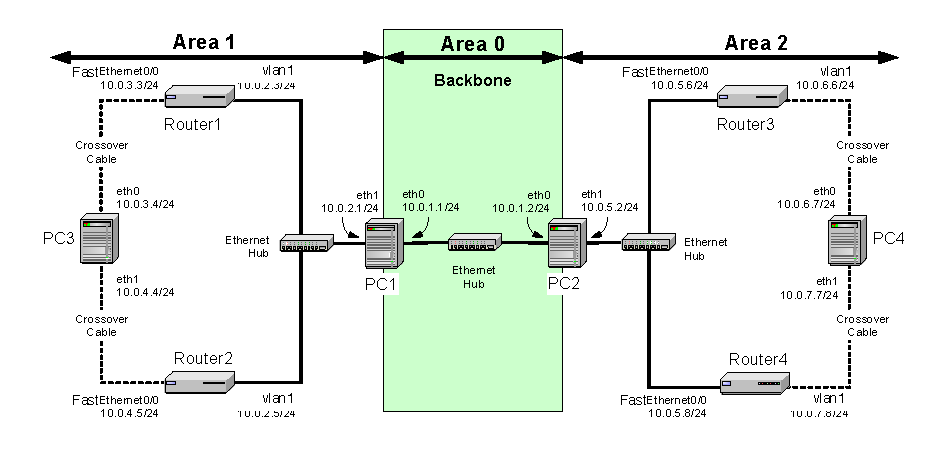
\includegraphics[width=\linewidth]{graphics/lab4-network2-part5-updated.pdf}	
	\caption{Network configuration for Part 5}
	\label{fig:lab4-network2-part5}
\end{figure}

In the following exercises you define the areas, and then observe how the link state databases are built.

\subsubsection*{Exercise 5. Defining multiple areas in OSPF}

\begin{enumerate}
	\item Restart the \cmd{zebra} and \cmd{ospfd} processes on all four Linux PCs. Use the same \path{daemons} configuration file as used in the previous exercise.
		\begin{cmdblock}
	PC1% /etc/init.d/quagga restart
		\end{cmdblock}
	\item Start Wireshark on PC1 and capture traffic on interface \iface{eth0}.
	\item Change the Area IDs of the Cisco routers and the PCs. On each system, the directly connected networks are assigned to an area with a 24-bit prefix. Here are the configurations for PC3, PC1, and Router 1. The other configurations are similar.
		PC3, which belongs to only one area, is configured as follows:
		\begin{cmdblock}
	PC3% telnet localhost 2604 Password: <login password>
	ospfd> enable
	ospfd# configure terminal
	ospfd(config)# router ospf 
	ospfd(config-router)# router-id 10.0.3.4 
	ospfd(config-router)# network 10.0.3.0/24 area 1 
	ospfd(config-router)# network 10.0.4.0/24 area 1 
	ospfd(config-router)# end
	ospfd# exit
		\end{cmdblock}
		PC1, belongs to two areas, and is configured as follows:
		\begin{cmdblock}
	PC1% telnet localhost 2604 Password: <login password>
	ospfd> enable
	ospfd# configure terminal
	ospfd(config)# router ospf 
	ospfd(config-router)# router-id 10.0.1.1 
	ospfd(config-router)# network 10.0.2.0/24 area 1 
	ospfd(config-router)# network 10.0.1.0/24 area 0 
	ospfd(config-router)# end
	ospfd# exit
		\end{cmdblock}
		The configuration of Router 1 is as follows:
		\begin{cmdblock}
	Router1# configure terminal
	Router1(config)# no router ospf 1
	Router1(config)# router ospf 1
	Router1(config-router)# network 10.0.3.0 0.0.0.255 area 1
	Router1(config-router)# network 10.0.2.0 0.0.0.255 area 1 
	Router1(config-router)# end
	Router1# clear ip ospf 1 process
		\end{cmdblock}
	\item Once the routing tables have converged, test the network configuration with the commands \cmd{traceroute} and \cmd{ping} on the Linux PCs, and the commands trace and ping on the Cisco routers. All hosts and routers should be able to communicate with each other.
	\item Save the link state database on all Cisco routers and on all Linux PCs. On the Linux PCs, open a Telnet session to the ospfd process, and then type
		\begin{cmdblock}
	ospfd# show ip ospf database router
		\end{cmdblock}
		On the Cisco routers, type
		\begin{cmdblock}
	Router1# show ip ospf database
		\end{cmdblock}
		Save the output of the link state databases to a file.
\end{enumerate}

\begin{questions}
	\q{5.1.a}{Refer to the saved link state databases in your answers. Compare the link state databases to those saved in Part 4. Which differences do you note?}
	\q{5.1.b}{Which information do routers in Area 1 have about Area 2? Which information do they have about the backbone area (Area 0)?}
	\q{5.1.c}{How much information do the routers in the backbone area (Area 0) have about the topology of Area 1 and Area 2?}
	\q{5.1.d}{How do the IP routers in Area 1 know how to forward traffic to Area 2?}
\end{questions}

\begin{enumerate}[resume]
	\item Display the area routers known to Router 1 from Area 1, with the command
		\begin{cmdblock}
	Router1# show ip ospf border-routers
		\end{cmdblock}
		Save the output to a file.
	\item Save the Wireshark output of OSPF packet types (selecting the Print Detail option) that you did not observe in Part 4. Only include one packet of each type.
\end{enumerate}

\begin{questions}
	\q{5.2}{Include the Wireshark output in your report showing, if any, the different types of OSPF packets that you did not observe in Part 5.}
	\q{5.3}{Include the output of the link state databases saved in Step 5.}
	\q{5.4}{Explain the output of the command ``show ip ospf border-routers'' in Step 6.}
\end{questions}
